\PassOptionsToPackage{unicode}{hyperref}
\documentclass[aspectratio=1610, 11pt]{beamer}

\usepackage{amsmath}
\usepackage{amssymb}
\usetheme{tudo}

\title{Datenstrukturen, Algorithmen und Programmierung~2}
\author[A.~Coja-Oghlan]{Amin Coja-Oghlan}
\institute[DAP2]{Lehrstuhl Informatik 2\\Fakult\"at f\"ur Informatik}

\newcommand\dist{\mathrm{dist}}
\renewcommand{\vec}[1]{\boldsymbol{#1}}
\newcommand\NULL{{\tt NULL}}
\newcommand\dd{\mathrm d}
\newcommand\eul{\mathrm e}
\newcommand\cA{\mathcal A}
\newcommand\cB{\mathcal B}
\newcommand\cC{\mathcal C}
\newcommand\cD{\mathcal D}
\newcommand\cE{\mathcal E}
\newcommand\cF{\mathcal F}
\newcommand\cG{\mathcal G}
\newcommand\cH{\mathcal H}
\newcommand\cI{\mathcal I}
\newcommand\cJ{\mathcal J}
\newcommand\cK{\mathcal K}
\newcommand\cL{\mathcal L}
\newcommand\cM{\mathcal M}
\newcommand\cN{\mathcal N}
\newcommand\cO{\mathcal O}
\newcommand\cP{\mathcal P}
\newcommand\cQ{\mathcal Q}
\newcommand\cR{\mathcal R}
\newcommand\cS{\mathcal S}
\newcommand\cT{\mathcal T}
\newcommand\cU{\mathcal U}
\newcommand\cV{\mathcal V}
\newcommand\cW{\mathcal W}
\newcommand\cX{\mathcal X}
\newcommand\cY{\mathcal Y}
\newcommand\cZ{\mathcal Z}
\newcommand\fA{\mathfrak A}
\newcommand\fB{\mathfrak B}
\newcommand\fC{\mathfrak C}
\newcommand\fD{\mathfrak D}
\newcommand\fE{\mathfrak E}
\newcommand\fF{\mathfrak F}
\newcommand\fG{\mathfrak G}
\newcommand\fH{\mathfrak H}
\newcommand\fI{\mathfrak I}
\newcommand\fJ{\mathfrak J}
\newcommand\fK{\mathfrak K}
\newcommand\fL{\mathfrak L}
\newcommand\fM{\mathfrak M}
\newcommand\fN{\mathfrak N}
\newcommand\fO{\mathfrak O}
\newcommand\fP{\mathfrak P}
\newcommand\fQ{\mathfrak Q}
\newcommand\fR{\mathfrak R}
\newcommand\fS{\mathfrak S}
\newcommand\fT{\mathfrak T}
\newcommand\fU{\mathfrak U}
\newcommand\fV{\mathfrak V}
\newcommand\fW{\mathfrak W}
\newcommand\fX{\mathfrak X}
\newcommand\fY{\mathfrak Y}
\newcommand\fZ{\mathfrak Z}
\newcommand\fa{\mathfrak a}
\newcommand\fb{\mathfrak b}
\newcommand\fc{\mathfrak c}
\newcommand\fd{\mathfrak d}
\newcommand\fe{\mathfrak e}
\newcommand\ff{\mathfrak f}
\newcommand\fg{\mathfrak g}
\newcommand\fh{\mathfrak h}
%\newcommand\fi{\mathfrak i}
\newcommand\fj{\mathfrak j}
\newcommand\fk{\mathfrak k}
\newcommand\fl{\mathfrak l}
\newcommand\fm{\mathfrak m}
\newcommand\fn{\mathfrak n}
\newcommand\fo{\mathfrak o}
\newcommand\fp{\mathfrak p}
\newcommand\fq{\mathfrak q}
\newcommand\fr{\mathfrak r}
\newcommand\fs{\mathfrak s}
\newcommand\ft{\mathfrak t}
\newcommand\fu{\mathfrak u}
\newcommand\fv{\mathfrak v}
\newcommand\fw{\mathfrak w}
\newcommand\fx{\mathfrak x}
\newcommand\fy{\mathfrak y}
\newcommand\fz{\mathfrak z}
\newcommand\vA{\vec A}
\newcommand\vB{\vec B}
\newcommand\vC{\vec C}
\newcommand\vD{\vec D}
\newcommand\vE{\vec E}
\newcommand\vF{\vec F}
\newcommand\vG{\vec G}
\newcommand\vH{\vec H}
\newcommand\vI{\vec I}
\newcommand\vJ{\vec J}
\newcommand\vK{\vec K}
\newcommand\vL{\vec L}
\newcommand\vM{\vec M}
\newcommand\vN{\vec N}
\newcommand\vO{\vec O}
\newcommand\vP{\vec P}
\newcommand\vQ{\vec Q}
\newcommand\vR{\vec R}
\newcommand\vS{\vec S}
\newcommand\vT{\vec T}
\newcommand\vU{\vec U}
\newcommand\vV{\vec V}
\newcommand\vW{\vec W}
\newcommand\vX{\vec X}
\newcommand\vY{\vec Y}
\newcommand\vZ{\vec Z}
\newcommand\va{\vec a}
\newcommand\vb{\vec b}
\newcommand\vc{\vec c}
\newcommand\vd{\vec d}
\newcommand\ve{\vec e}
\newcommand\vf{\vec f}
\newcommand\vg{\vec g}
\newcommand\vh{\vec h}
\newcommand\vi{\vec i}
\newcommand\vj{\vec j}
\newcommand\vk{\vec k}
\newcommand\vl{\vec l}
\newcommand\vm{\vec m}
\newcommand\vn{\vec n}
\newcommand\vo{\vec o}
\newcommand\vp{\vec p}
\newcommand\vq{\vec q}
\newcommand\vr{\vec r}
\newcommand\vs{\vec s}
\newcommand\vt{\vec t}
\newcommand\vu{\vec u}
\renewcommand\vv{\vec v}
\newcommand\vw{\vec w}
\newcommand\vx{\vec x}
\newcommand\vy{\vec y}
\newcommand\vz{\vec z}
\renewcommand\AA{\mathbb A}
\newcommand\NN{\mathbb N}
\newcommand\ZZ{\mathbb Z}
\newcommand\PP{\mathbb P}
\newcommand\QQ{\mathbb Q}
\newcommand\RR{\mathbb R}
\newcommand\RRpos{\mathbb R_{\geq0}}
\newcommand\QQpos{\mathbb Q_{\geq0}}
\renewcommand\SS{\mathbb S}
\newcommand\CC{\mathbb C}
\newcommand{\ord}{\mathrm{ord}}
\newcommand{\id}{\mathrm{id}}
\newcommand{\pr}{\mathrm{P}}
\newcommand{\Vol}{\mathrm{vol}}
\newcommand\norm[1]{\left\|{#1}\right\|} 
\newcommand\sign{\mathrm{sign}}
\newcommand{\eps}{\varepsilon}
\newcommand{\abs}[1]{\left|#1\right|}
\newcommand\bc[1]{\left({#1}\right)} 
\newcommand\cbc[1]{\left\{{#1}\right\}} 
\newcommand\bcfr[2]{\bc{\frac{#1}{#2}}} 
\newcommand{\bck}[1]{\left\langle{#1}\right\rangle} 
\newcommand\brk[1]{\left\lbrack{#1}\right\rbrack} 
\newcommand\scal[2]{\bck{{#1},{#2}}} 
\newcommand{\vecone}{\mathbb{1}}
\newcommand{\tensor}{\otimes}
\newcommand{\diag}{\mathrm{diag}}
\newcommand{\ggt}{\mathrm{ggT}}
\newcommand{\kgv}{\mathrm{kgV}}
\newcommand{\trans}{\top}
\newcommand{\Karonski}{Karo\'nski}
\newcommand{\Erdos}{Erd\H{o}s}
\newcommand{\Renyi}{R\'enyi}
\newcommand{\Lovasz}{Lov\'asz}
\newcommand{\Juhasz}{Juh\'asz}
\newcommand{\Bollobas}{Bollob\'as}
\newcommand{\Furedi}{F\"uredi}
\newcommand{\Komlos}{Koml\'os}
\newcommand{\Luczak}{\L uczak}
\newcommand{\Kucera}{Ku\v{c}era}
\newcommand{\Szemeredi}{Szemer\'edi}

\newcommand{\mytitle}{AVL-B\"aume}

\begin{document}

\frame[plain]{\titlepage}

\begin{frame}\frametitle{\mytitle}
	\begin{exampleblock}{Worum geht es?}
		\begin{itemize}
			\item AVL-B\"aume, benannt nach ihren Erfindern Adelson-Velsky und Landis sind eine Alternative zu rot-schwarz-B\"aumen
			\item alle Operationen ben\"otigen Zeit $O(\log n)$
			\item wiederum m\"ussen wir die Operationen ``einf\"ugen'' und ``entfernen'' anpassen
		\end{itemize}
	\end{exampleblock}
\end{frame}

\begin{frame}\frametitle{\mytitle}
	\begin{block}{Definition}
		Ein AVL-Baum ist ein gewurzelter bin\"arer Suchbaum, in dem sich f\"ur jeden Knoten $v$ die H\"ohe des linken und des rechten Teilbaums um h\"ochstens eins unterscheidet.
	\end{block}
	\begin{exampleblock}{}
		\begin{itemize}
			\item folglich haben AVL-B\"aume H\"ohe $O(\log n)$
			\item somit haben die Operationen {\tt Search}, {\tt Minimum}, {\tt Maximum}, {\tt Successor}, {\tt Predecessor} Laufzeit $O(\log n)$
		\end{itemize}
	\end{exampleblock}
\end{frame}

\begin{frame}\frametitle{\mytitle}
	\begin{exampleblock}{H\"ohenbalance}
		\begin{itemize}
			\item um die AVL-Definition zu erhalten, f\"ugen wir jedem Knoten des Baumes ein weiteres Datenelement hinzu
			\item dieser zus\"atzliche Eintrag ist die {\em H\"ohe} des Teilbaums, der an diesem Knoten ``h\"angt''
			\item genauer gesagt gen\"ugt die \alert{Balance}
				\begin{align*}
					\beta(v)&=\mbox{H\"ohe des rechten Teilbaums von $v$}-\mbox{H\"ohe des linken Teilbaums von $v$}.
				\end{align*}
		\end{itemize}
	\end{exampleblock}
\end{frame}

\begin{frame}\frametitle{\mytitle}
	\begin{exampleblock}{H\"ohenbalance}
		\begin{itemize}
			\item wir f\"ugen zun\"achst einen neuen Knoten $z$ wie in einen gew\"ohnlichen bin\"aren Suchbaum ein
			\item dadurch kann allerdings die AVL-Eigenschaft zerst\"ort werden
			\item um sie wiederherzustellen, f\"uhren wir geeignete \alert{Rotationen}
			\item diese werden \alert{rekursiv} von unten nach oben auf dem Pfad zur Wurzel ausgef\"uhrt
			\item dabei bezeichnet $\beta$ auf die Balance {\em vor} dem Einf\"ugen des neuen Knotens $z$
		\end{itemize}
	\end{exampleblock}
\end{frame}

\begin{frame}\frametitle{\mytitle}
	\begin{exampleblock}{Balancieren nach Einf\"ugen}
		\begin{enumerate}
			\item falls $z$ die Wurzel ist, halte; sonst sei $p$ der Elternknoten von $z$.
			\item falls $z$ das rechte Kind von $p$ ist
			\item $\quad$falls $\beta(p)>0$
			\item $\qquad$falls $\beta(z)<0$
			\item $\quad\qquad$Rechtsrotation um $z$, anschlie\ss end Linksrotation um $p$
			\item $\qquad$sonst Linksrotation um $p$
			\item $\quad$sonst
			\item $\qquad$falls $\beta(p)<0$, setze $\beta(p)=0$ und halte
			\item $\qquad$sonst setze $\beta(p)=1$
			\item \itshape sonst verfahre analog wie oben mit links/rechts vertauscht
		\end{enumerate}
	\end{exampleblock}
\end{frame}

\begin{frame}\frametitle{\mytitle}
	\begin{overprint}
		\onslide<1>\hfill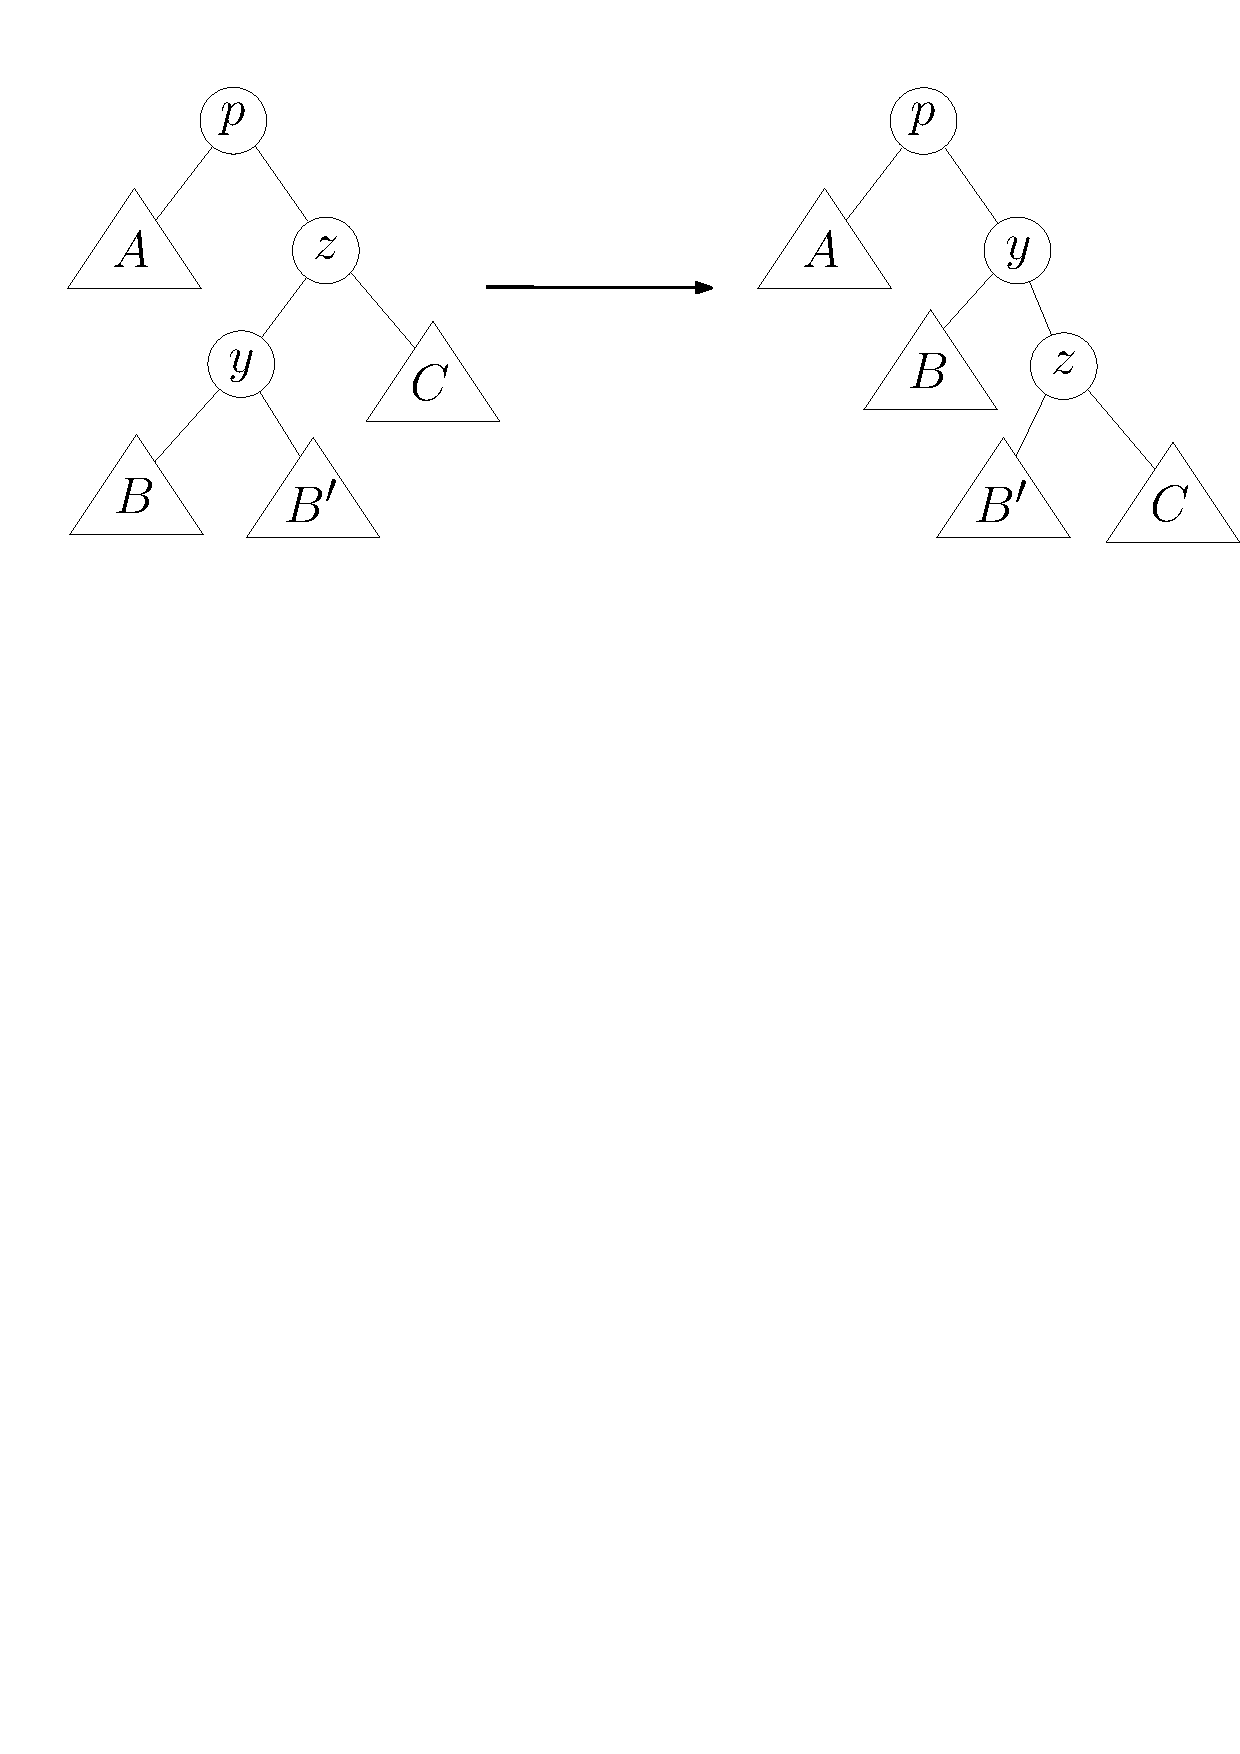
\includegraphics[height=30mm]{./images/avl_insert_rightleft1.pdf}
		\onslide<2>\hfill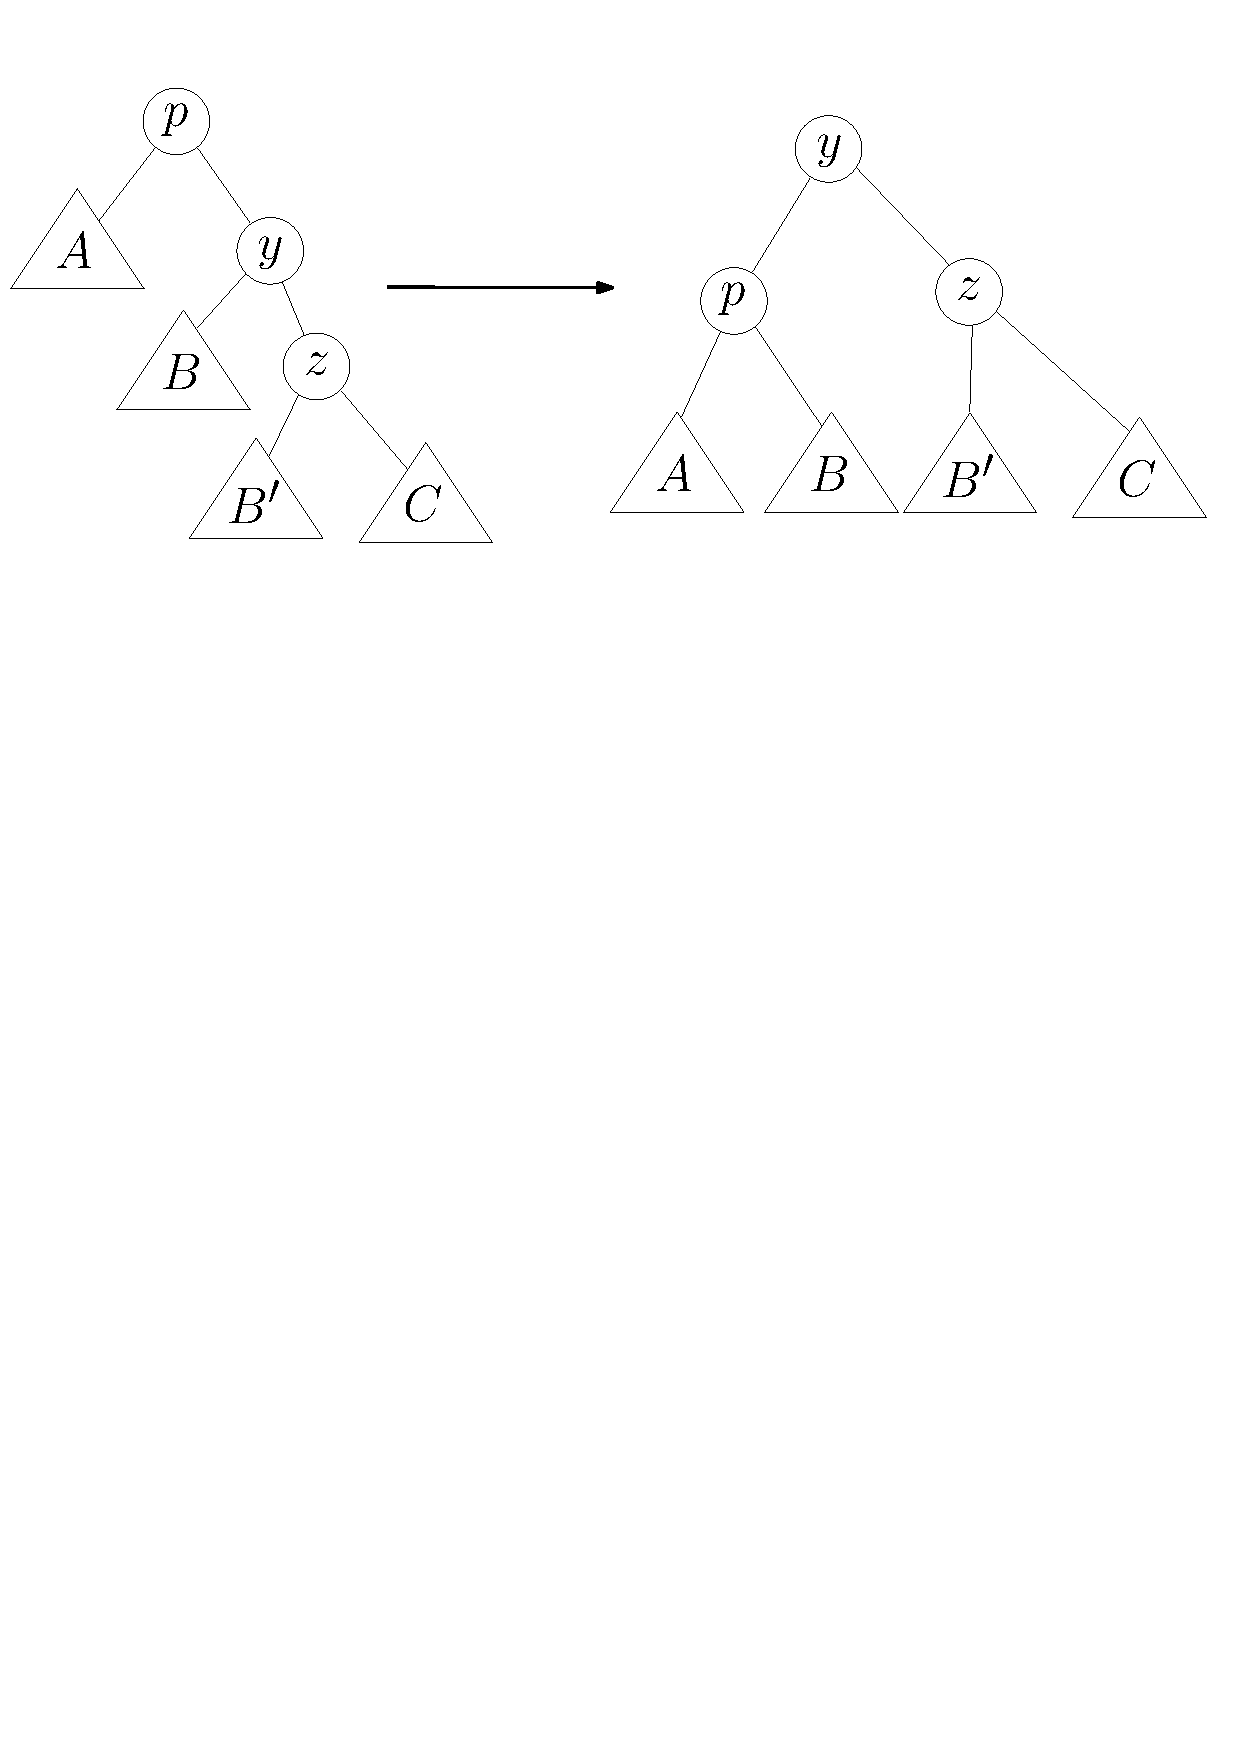
\includegraphics[height=30mm]{./images/avl_insert_rightleft2.pdf}
	\end{overprint}
	\begin{exampleblock}{$\beta(p)>0$ und $\beta(z)<0$}
		\begin{itemize}
			\item Rechtsrotation um $z$
			\item dann Linksrotation um $p$
		\end{itemize}
	\end{exampleblock}
\end{frame}

\begin{frame}\frametitle{\mytitle}
	\hfill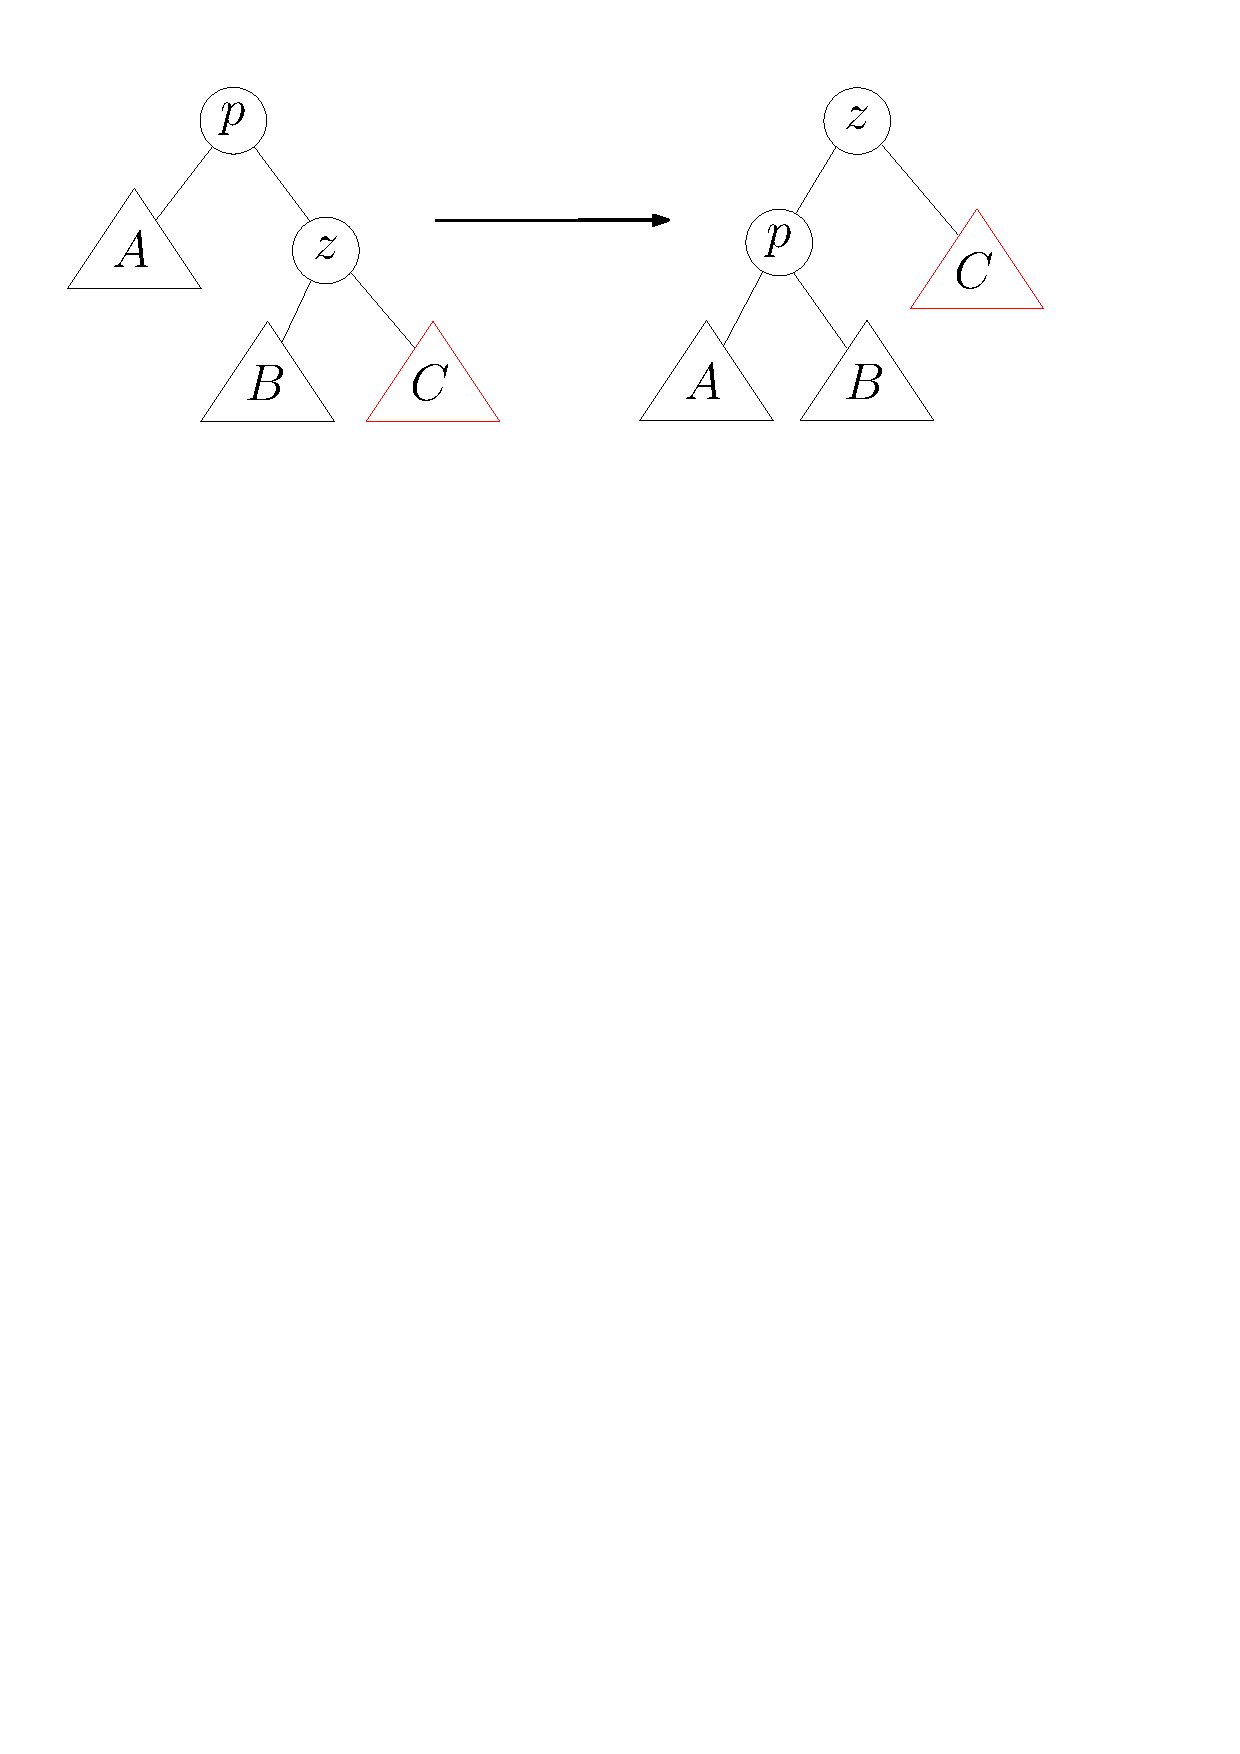
\includegraphics[height=30mm]{./images/avl_insert_left.pdf}
	\begin{exampleblock}{$\beta(p)>0$ und $\beta(z)\geq0$}
		\begin{itemize}
			\item Linksrotation um $p$
		\end{itemize}
	\end{exampleblock}
\end{frame}

\begin{frame}\frametitle{\mytitle}
	\begin{exampleblock}{Balancieren nach L\"oschen}
		\begin{enumerate}
			\item falls $z$ die Wurzel ist, halte.
			\item sei $p$ der Elternknoten von $z$ und $y$ der Schwesterkonten von $z$ (bzw.\ $y=\emptyset$)
			\item falls $z$ das linke Kind von $p$ ist
			\item $\quad$falls $\beta(p)>0$
			\item $\qquad$falls $\beta(y)<0$
			\item $\quad\qquad$Rechtsrotation um $y$, anschlie\ss end Linksrotation um $p$
			\item $\qquad$sonst Linksrotation um $p$
			\item $\quad$sonst
			\item $\qquad$falls $\beta(p)=0$, setze $\beta(p)=1$ und halte
			\item $\qquad$sonst setze $\beta(p)=0$ %und balanciere rekursiv $(T,r,p)$
			\item \itshape sonst verfahre analog wie oben mit links/rechts vertauscht
		\end{enumerate}	
	\end{exampleblock}
\end{frame}

\begin{frame}\frametitle{\mytitle}
	\begin{exampleblock}{Zusammenfassung}
		\begin{itemize}
			\item AVL-B\"aume sind eine Alternative zu rot-schwarz-B\"aumen
			\item Balancieroperation verwendet ausschlie\ss lich Rotationen
		\end{itemize}	
	\end{exampleblock}
\end{frame}

\end{document}
